\section{Evaluation}

\subsection{Training Datasets}
The datasets chosen for training are ideally clean, uniform and have about an equal number of each class instance. 

The system depends on the ability of the machine learning agent to be able to
match between acoustic features and the text queries. Its performance depends on
both the size of the database and the specificity of the query. To examine
performance across environments, we choose a clean and a dirty database: ESC-50
\cite{Piczak2015} and Freesound.

\subsubsection{ESC-50}
This clean database is made available on GitHub for environmental sound
classification. It is maintained such that the tag vocabulary is fixed and each
audio document attempts to only contains a single object in it. Each document is
5 seconds long and audio quality in terms of samplerate and recording noise is
normalized across the database. This makes for a very clean database with little
noise in both audio and annotation. It has 50 semantic classes with 40 examples
per class arranged into 5 major categories. However, the major categories do not
match the Gaver taxonomy and so were manually separated as in Table
~\ref{tab:relabel}. The database's sound documents come from the Freesound
project with the author providing uniform tags and normalizing the audio
manually \cite{Font2013}.

\subsubsection{Freesound}

\subsection{Results}

\subsubsection{Encoding Results}
\begin{figure}[h]
    \centering
    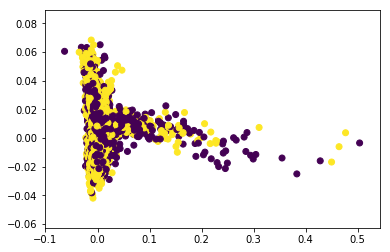
\includegraphics[width=0.45\textwidth]{figures/pca-cluster-hl.png}
    \caption{2D clustering of features using PCA.}
    \label{fig:pcahl}
\end{figure}

\begin{table}[t]
    \centering
    \begin{tabular}{c|cc}
    \textbf{Window} & \textbf{Read} & \textbf{Process} \\ \hline
    250              & 7840           & 37318                    \\
    2000             & 2413           & 4831                   
    \end{tabular}
    \caption{The average read and processing time in ms for 400 documents.}
    \label{tab:base-time}
\end{table}

\subsubsection{Training Evaluation}

\begin{figure}
    \centering
    \includegraphics[width=0.45\textwidth]{example-image-a}
    \caption{Comparative training time between PAMIR, WARP, and ECHO (what we're calling this system?)}
    \label{fig:my-label}
\end{figure}

\begin{figure}
    \centering
    \includegraphics[width=0.45\textwidth]{example-image-a}
    \caption{Plot of training iterations needed before getting diminishing returns (comparative between classifiers)}
    \label{fig:learning-curve}
\end{figure}

\subsubsection{Representation Experiments}

\begin{table}[]
    \begin{tabular}{llllll}
    Classifier/Window       & 250 ms & 500 ms & 1 s   & 2 s  & 5 s   \\
    Deep Neural Nets        & 0.628  & 0.653  & 0.656 &      &       \\
    Random Forest           & 0.663  & 0.663  &       & 0.77 & 0.76  \\
    K-Nearest Neighbors     &        &        &       &      & 0.725 \\
    Support Vector Machine  &        &        &       & 0.70 & 0.71  \\
    Gaussian Mixtures Model &        &        &       &      &      
    \end{tabular}
\end{table}

Classifier performance at different window sizes and features (remember, have run wavenet)

\subsubsection{Pure Classification Performance}

Cross-validated performance of each subclassifier and performance of hierarchical

\subsubsection{Retrieval Performance (Time + Accuracy)}

% \subsubsection{Encoding}

% These experiments attempted to measure the effectiveness of different encoding
% approaches as well as a base case of an extracted feature vector. Audio is read
% in using a blocksize of 2s or 250ms with overlap of 1s and 125ms respectively.
% This is done to determine effective time windowing of the data, however this
% approach added some overhead for reading of files as summarized in Table
% ~\ref{tab:base-time}. A more granular blocksize causes the read and processing
% time to greatly increase, because of the increase in individual audio clips
% being evaluated.

% \subsubsection{Extracted Features}
% This representation of the audio was created using feature extraction techniques
% found in the librosa library \cite{brian-mcfee-2018-1252297}. The features
% chosen for classification as a base case were the first 13 MFCCs and the
% spectral contrast of the signal. MFCCs are common in audio classification tasks
% as they are often able to keep much of the signal's information without needing
% the entire spectrogram. The first and second derivative of MFCCs were also
% computed for the feature vector to provide the learner with some features that
% can emulate how the signal changes over time. To this end, spectral contrast is
% also added as it provides the contrast between the peaks and valleys of the
% signal at each frame. The extracted features are then averaged down to a single
% vector per frame. In all, the feature vector is made up of 49 values.

% \subsubsection{Neural Network}
% As mentioned before, it is common to use an auto-encoder to create latent
% variables for classification. The idea is similar to that of a clustering
% algorithm like Principal Components Analysis in which the algorithm tries to
% find features that are of greatest variance. Here, both traditional neural
% networks and convolutional neural networks are used to create an encoder. The
% overall results were underwhelming with the biggest gain being made on the
% testing set. In all these auto-encoders provided about +/- 5\% accuracy change
% which can also be attributed to shuffling of data during training. The results
% of the auto-encoding with CNNs are summarized in Figure ~\ref{fig:encode}. Here,
% frames of audio are converted into expanded representations with more weight
% given to the most recent frame so the encoder can learn temporal relationships.
% It appears to learn a latent representation well with a reconstruction score of
% approximately 47\%. However, the auto-encoder takes between 45 and 75 minutes to
% fully train and the results are no better than previous.

% \subsubsection{Classification}

% \begin{table}[t]
%     \begin{tabular}{lll}
%         & 250ms   & 2000ms  \\ \hline
%     SVM & 0.627 & 0.622 \\
%     SNN & 0.717 & 0.729 \\
%     RFC & 0.688 & 0.665
%     \end{tabular}
%     \caption{Classifier precision for top level.}
%     \label{tab:topacc}
% \end{table}


% \subsubsection{Top Level Classifier}

% As described previously, this classifier is meant to discriminate between the
% highest level of the Gaver taxonomy. Table ~/ref{tab:topacc} summarizes the
% precision of each of these classifiers for the different blocksizes. Figure
% ~\ref{fig:TopClass} shows the confusion matrix of the most accurate model for
% each classifier as there was little difference between the blocksizes. The
% experiments show that the shallow network approach provides the best
% approximation of the two classes. SVMs were the poorest performers at 63\%
% accuracy at maximum with most guesses being for interacting materials. In this
% case, it is likely that the features used for evaluation were not linearly
% differentiable and thus the standard SVM was unable to find a good decision
% boundary. RFCs and SNNs performed similar in this task with the SNN giving
% slightly more weight to interacting elements than the RFC.

% \begin{table}[t]
%     \caption{Classifier precision for \textit{Animal Voices}.}
%     \label{tab:animvocprec}
%     \begin{tabular}{lll}
%         & 250   & 2000  \\ \hline
%     SVM & 0.069 & 0.073 \\
%     DNN & 0.280 & 0.300 \\
%     RFC & 0.254 & 0.212
%     \end{tabular}
% \end{table}

% \begin{figure}[t]
%     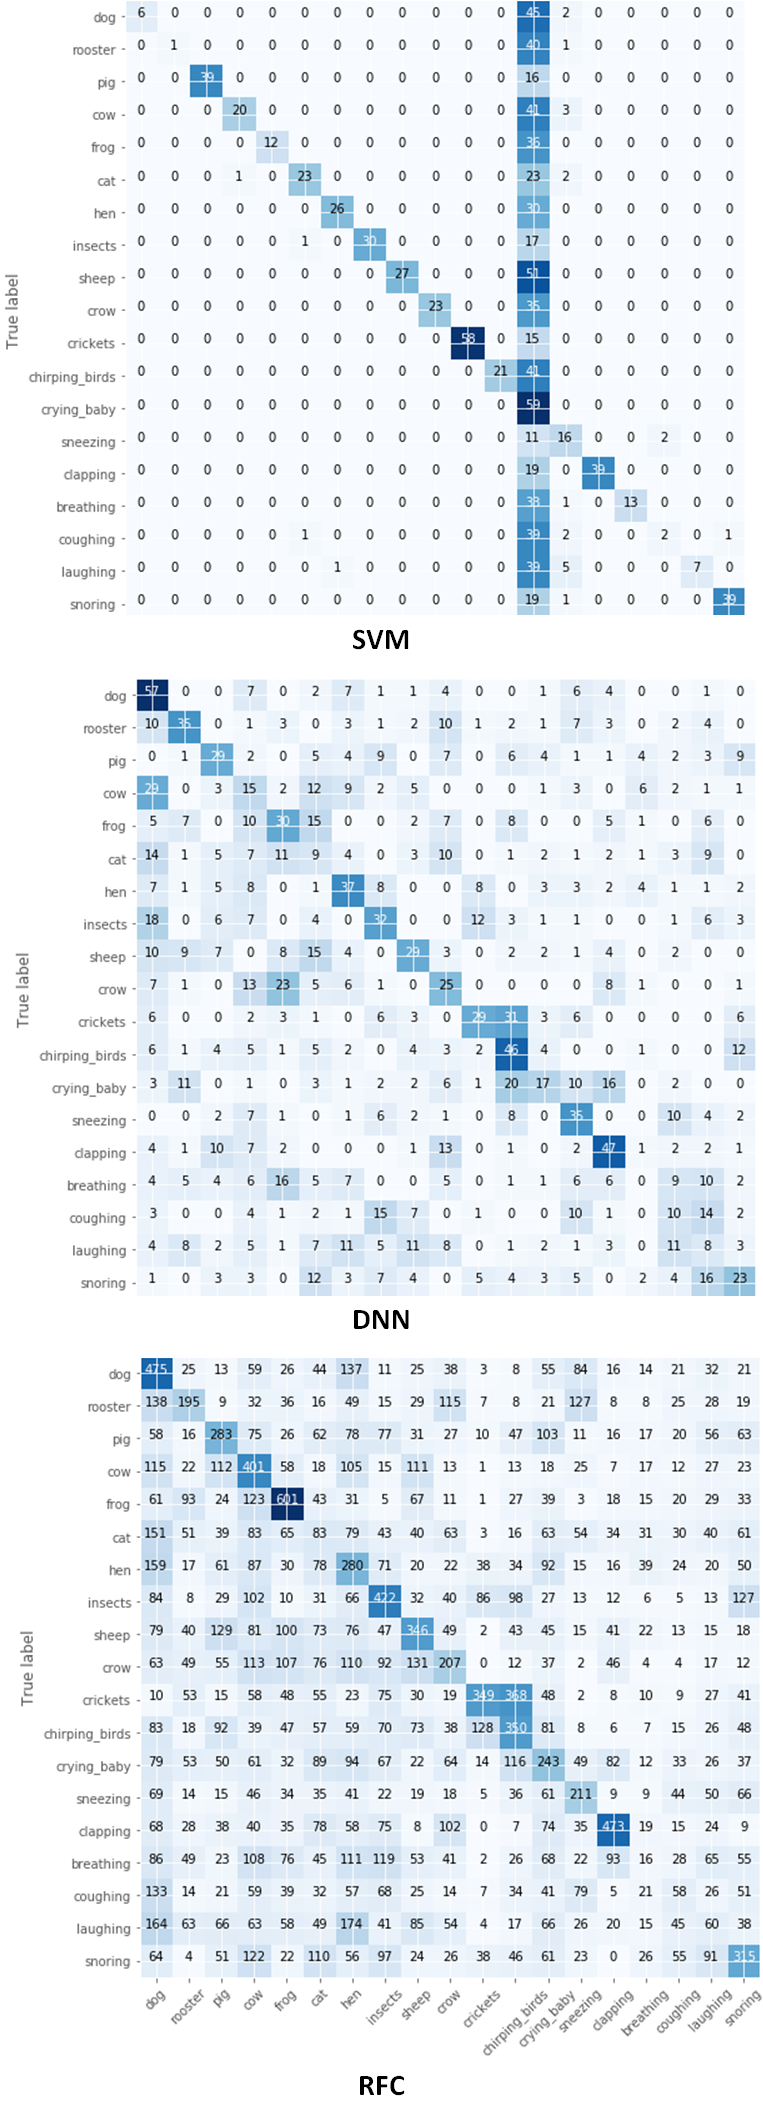
\includegraphics[width=0.3\textwidth]{figures/Animal-Classification-Comparison.png}
%     \caption{Summary of classification results for the \textit{Animal Voices} classifier.}
%     \label{fig:AnimClass}
% \end{figure}

% \subsubsection{Animal Voices Classifier}

% The classifier is trained on the 19 classes identified beforehand. The 19
% classes that make up the animal sounds in the database have some overlap,
% especially for identifiers like "breathing" and "laughing" as these are often
% breathy sounds. The precision results of each classifier is summarized in Table
% ~\ref{tab:animvocprec}. Here, DNNs outperform both classifiers on precision
% however with a 2 second time window we see DNN achieve its maximum precision
% while RFC precision decreases.

% The confusion matrices in Figure ~\ref{fig:AnimClass} illustrates the agent
% often misclassifies breathing, coughing, laughing, and snoring across nearly
% every other class. This phenomenon is illustrated by the cutout in Figure
% ~\ref{fig:breath}. The highest concentration of false predictions of these four
% classes occurs between the classes. It is believed that this is likely due to
% the sounds in the database invariably capturing the animal's breathing patterns
% which, in this case, trains the network on mislabeled breathing examples.

% \begin{figure}[t]
%     \centering
%     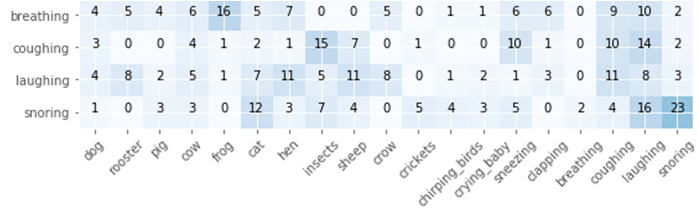
\includegraphics[width=0.45\textwidth]{figures/breathcorrelation.png}
%     \caption{A cutout of the \textit{Animal Voice} DNN matrix.}
%     \label{fig:breath}
% \end{figure}

% Another false correlation arose in this subset of the data, the agent is
% consistently confused between birds chirping and crickets. This is likely due to
% both the pitch and duration of the sounds being more similar to each other than
% to other sounds in the training set. This causes the agent to give less
% importance to these classes during training as committing neurons to them
% increases the loss elsewhere.

% \begin{table}[t]
%     \begin{tabular}{ccc}
%         & 250   & 2000  \\ \hline
%     SVM & 0.045 & 0.057 \\
%     DNN & 0.189 & 0.191 \\
%     RFC & 0.185 & 0.176
%     \end{tabular}
%     \caption{Classifier precision for \textit{Interacting Materials}.}
%     \label{tab:interactprec}
% \end{table}

% \begin{figure}[t]
%     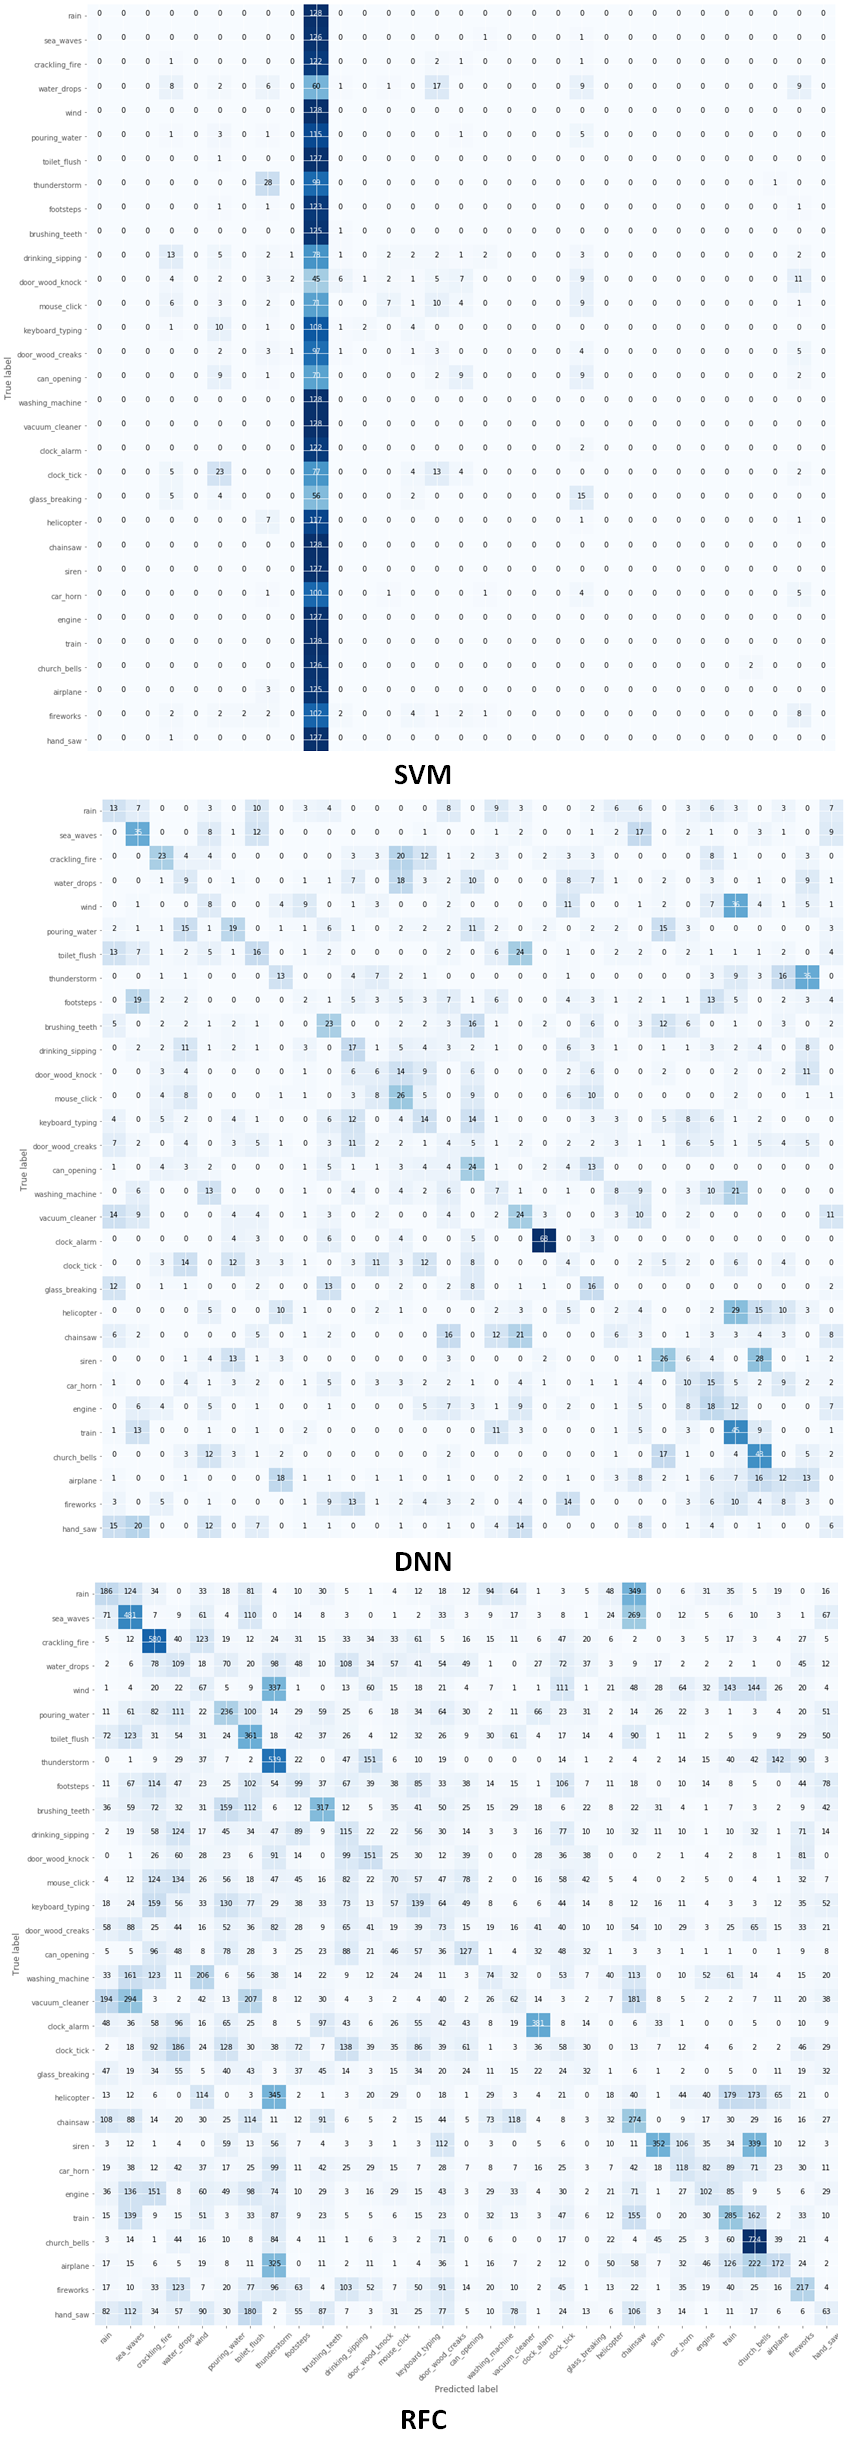
\includegraphics[width=0.3\textwidth]{figures/Material-Classification-Comparison.png}
%     \caption{Summary of classification results for the \textit{Interacting Materials} classifier.}
%     \label{fig:InterClass}
% \end{figure}

% \subsubsection{Interacting Materials}
% This classification task has 31 classes, with many having overlapping kinds of
% sounds. This is especially true of classes with flowing water which makes up
% 25\% of the data. As seen in Figure ~\ref{fig:InterClass} class confusion is
% widespread in DNNs though it is more densely concentrated than the results of
% the RFC. The hypothesis is that these confusions have a basis in the source and
% where the sound was recorded.

% In the results here we found that much of the class confusion was a result of
% the sound tags being ambiguous with regard to other classes. This is most
% apparent in classes that are in some way related to water. Here we have separate
% classes for pouring water, rain, sea waves, and water drops among others. The
% potential for confusion here is high as recordings with rain will invariably
% have examples of pouring water in them, similarly water drops are nearly
% synonymous with rain. Under this scrutiny, it is unsurprising that these classes
% were often confused for each other.

% Related to this phenomenon in \textit{Interacting Materials} is the occurrence
% of recordings containing overlapping sounds found elsewhere in the database. An
% example of this is the car horn class which understandably has audio documents
% that have a horn honking as the car is running. Since another detection target
% is engine, it is possible that blocks of audio from a car horn document will be
% classified as an engine. While this perception is correct, it is technically
% incorrect in the classification task and is marked as such. This kind of
% confusion is mitigated through our use of probabilistic ranking in results.

% \begin{table}[t]
%     \centering
%     \begin{tabular}{ccc}
%          & 250   & 2000  \\ \hline
%     DNN  & 0.174 & 0.191 \\
%     HDNN & 0.246 & 0.130
%     \end{tabular}
%     \caption{Classification results of a hierarchical DNN and a standard DNN trained on all 50 classes.}
%     \label{tab:overallprec}
% \end{table}


% \begin{figure}[t]
%     \caption{Resultant confusion matrix of HDNN model.}
%     \label{fig:Overall}
%     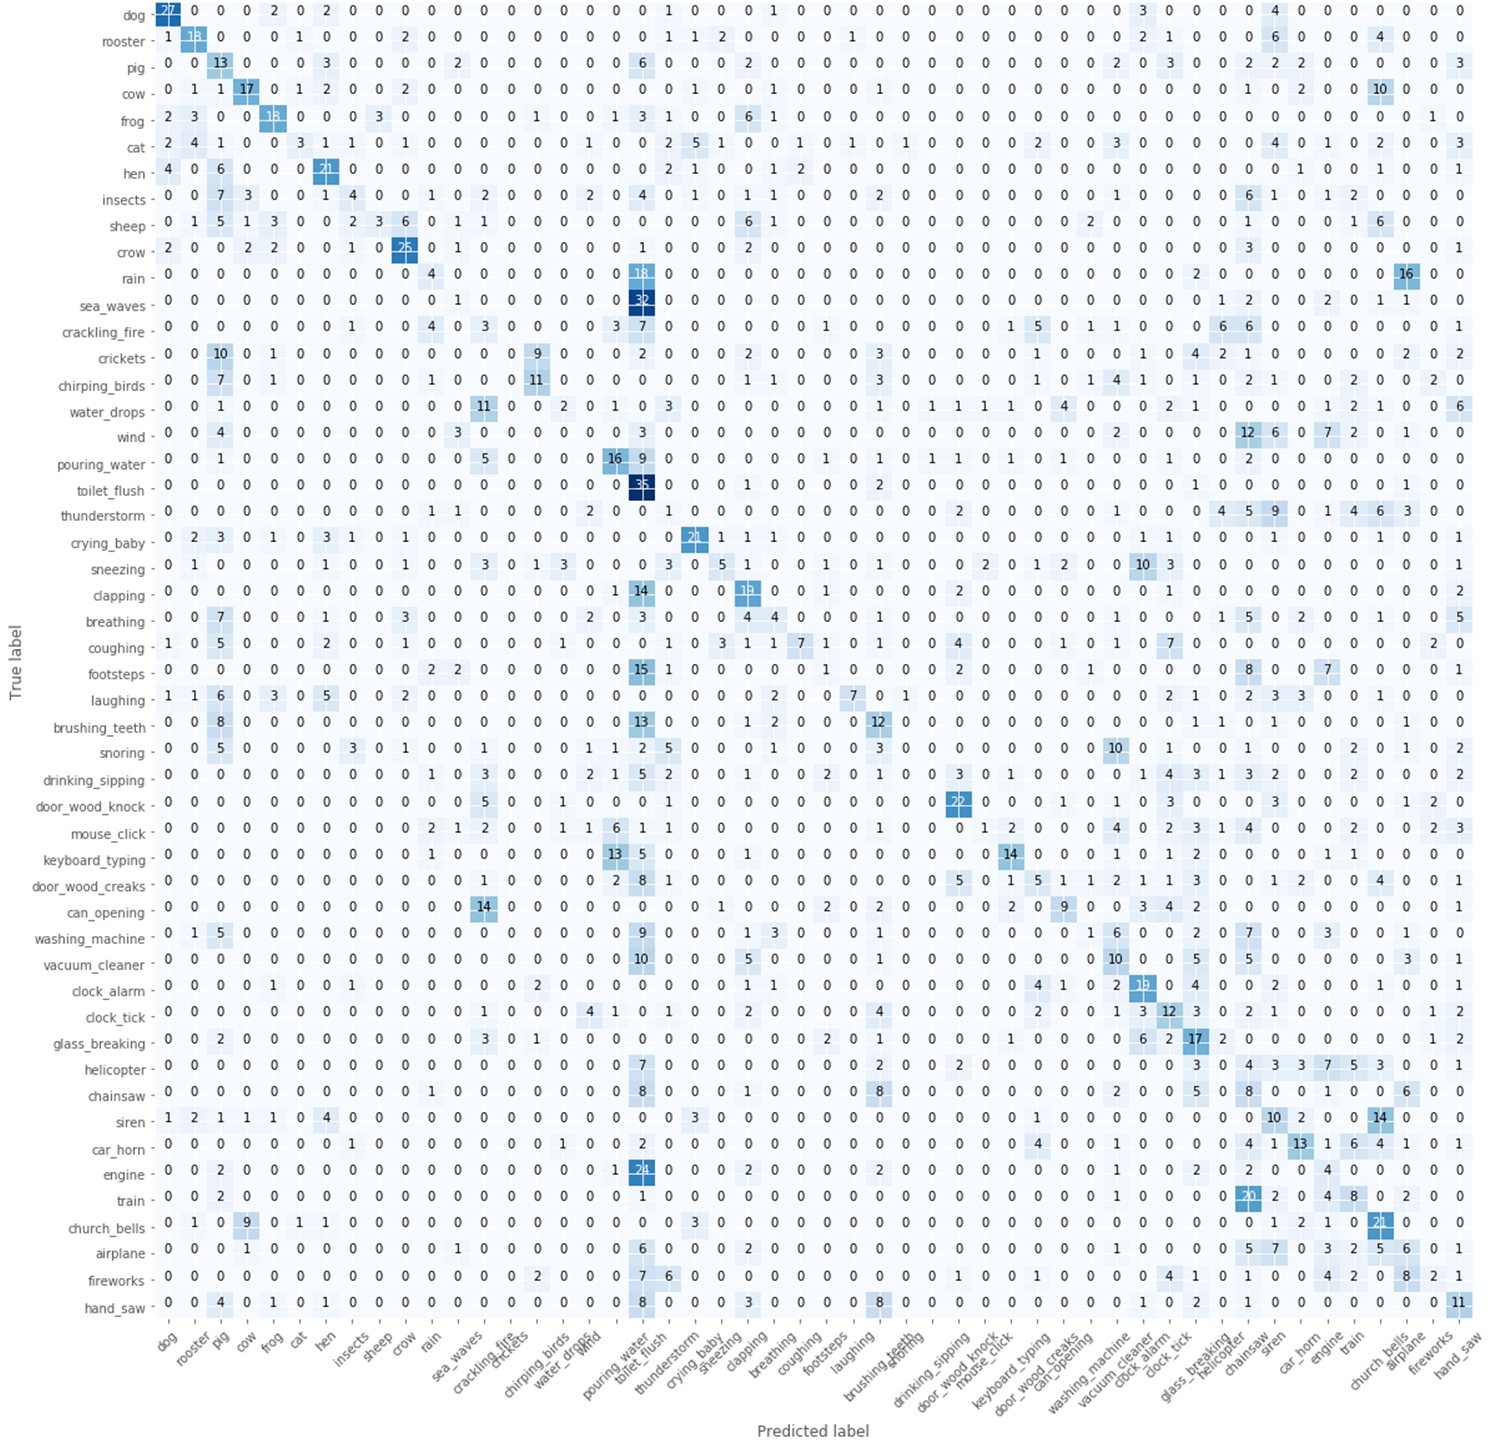
\includegraphics[width=0.40\textwidth]{figures/Overall.png}
% \end{figure}

% \subsubsection{Overall Accuracy}
% Here, we compare a DNN trained on all 50 classes at once to the hierarchical DNN
% (HDNN). The class of each document in the database is determined in the HDNN as
% the highest average probability class. It is important to note that this does
% not mean that all frames are equally certain of the class but that a majority
% considered it to be the correct class. As Table ~\ref{tab:overallprec} shows,
% the HDNN performs better when given more granular data on which to learn. This
% is likely a consequence of the learner having a more focused time window to
% better learn audio objects individually.

% Figure ~\ref{fig:Overall} illustrates a shortcoming of this prediction
% evaluation model. The line along the pouring water class is highly correlated to
% classes with water in them. It is likely that a majority of the audio document
% continuously has the sound of running water which is overwhelming the instances
% of the target class. This becomes even more clear when viewing the probability
% results of documents, it is often that the second-most probable class is the
% canonically correct class. This phenomenon is demonstrated by Figure
% ~\ref{fig:probChart}. In this case, it is unclear which should be taken as they
% have nearly equal probabilities but only one of them is technically correct.
% However, this is not as much of an issue when using this kind of classifier for
% retrieval as it is more important that a sound is detected in a document and not
% whether or not it is certainly the only sound in the document.

% \begin{figure}[t]
%     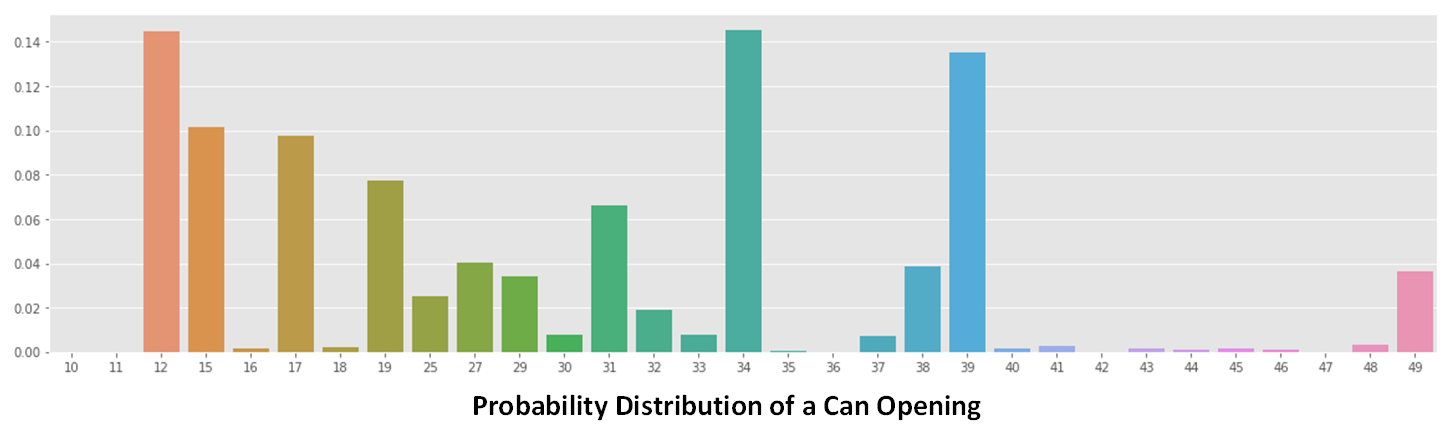
\includegraphics[width=0.50\textwidth]{figures/probchart.png}
%     \caption{Probability distribution of a can opening, the target class is 34 which here is tied for first.}
%     \label{fig:probChart}
% \end{figure}

\section{Conclusion}
The approach here shows promise, especially in the context of a retrieval
system. Using human perception as a model is an approach that had been pursued
in machine vision with success and it is only logical to do the same for machine
listening. By understanding the mechanisms by which we convert auditory signals
to brain signals, we can understand how the audio needs to be encoded for use in
machine hearing. One of the aspects of audio we have yet to optimally integrate
are temporal features which are of utmost importance in audio signals.

To this end, several representations were attempted in this work. The first was
just basic feature extraction from spectral representations of the audio using
librosa. Librosa allowed for many spectral and temporal features to be taken
from the signal though it is a slow process and may still not provide a good
feature set. To better emulate human perception, auto-encoders were attempted
next. The thought was that a neural network will be able to find latent
variables that are of better use than those extracted from usual means. However,
it was found that this approach did not bear out and hardly effected
performance.

Experiments were run comparing this approach to two off-the-shelf classifiers on
each layer of the hierarchy. The SVM classifier consistently under-performed and
will likely be removed from subsequent evaluations. A Random Forest Classifier
was consistently about equal to the neural networks it was evaluated against but
in nearly every case, the network was able to beat its precision score.

Overall, this study provided insights into the complexity of autonomous audio
analysis and the challenges that are still facing the field. of these
challenges, it seems that representation is the most pressing. It appears though
that the current direction of studying human perception mechanisms and emulating
them will prove optimal.